\chapter{Metodologia}
\label{sec:Metodologia}

Com o propósito de atingir o objetivo descrito na \autoref{sec:ObjetivoGeral}, o presente trabalho
realizou uma pesquisa exploratória acerca do tema abordado juntamente com a análise de alguns casos
práticos de empresas que fizeram a migração de uma arquitetura monolítica para uma arquitetura de
microsserviços, ou vice e versa. Assim, o desenvolvimento deste estudo baseou-se nas seguintes etapas:

\begin{description}
    \item [Etapa 1] Levantamento teórico inicial acerca dos objetos de análise diante dos
        referências teóricos adotados;
    \item [Etapa 2] Fichamento e agrupamento dos pontos de vista descobertos na Etapa 1, a fim de
        encontrar as perspectivas comuns e divergentes entre os autores estudados;
    \item [Etapa 3] Síntese acerca dos aspectos levantados sobre cada estilo arquitetural;
    \item [Etapa 4] Descrição e análise dos casos de estudo relevantes para o tema;
    \item [Etapa 5] Análise final comparando os dois modelos arquiteturais com base nos referencias
        teóricos adotados e nos casos práticos estudados.
\end{description}

A seguir serão apresentados os objetos de análise, as ferramentas utilizadas e a descrição de cada
etapa adotada. Vale ressaltar que deste ponto em diante alguns termos, como perspectivas ou
impactos, estarão destacados na presente seção com o intuito de chamar a devida atenção para o seu
significado, mas a frente será dada a definição tomada para cada um deles.

\section{Objetos de análise}
\label{sec:ObjetosDeAnalise}

Os objetos de análise pertinentes para o presente estudo consistem em:

    \begin{description}
        \item [Arquitetura monolítica:] estilo arquitetural tradicionalmente adotado em diversas
            empresas, no qual se detém uma base única de código.
        \item [Arquitetura de microsserviços:] estilo arquitetural distribuído, largamente adotado
            nos últimos anos por diversas empresas.
    \end{description}

\section{Ferramentas}

As ferramentas utilizadas para auxiliar na confecção do presente estudo foram:

\begin{description}
    \item[Miro] editor gráfico online que permite a construção de diagramas, mapa mentais, entre
        outros recursos gráficos relevantes ao conteúdo apresentado;
    \item[Google Planilhas] ferramenta para construção de tabelas.
    \item[Trello] quadro interativo que auxilia na organização de projetos utilizando do modelo
        Kanban.
\end{description}

\section{Descrição das etapas}
\subsection{Etapa 1 - Levantamento teórico}

A fundamentação teórica deste trabalho visou explorar os temas de arquitetura de software,
estilo arquitetural monolítico e estilo arquitetural de microsserviços por meio de livros, Google Scholar e
outras fontes de informação. Os tópicos abordados foram selecionados com base na sua respectiva
relevância dentro do assunto estudado e tiveram embasamento principalmente nos autores Martin Fowler,
Sam Newman, Mark Richards e Neal Ford, dentre outros.

\subsection{Etapa 2 - Perspectivas e aspectos}
\label{met:perspectivas}

Mediante a fundamentação teórica construída na Etapa 1, levantou-se os principais pontos acerca dos
estilos arquiteturais abordados que eram tratados pelos autores estudados, para tal utilizou-se da
ferramenta Trello com o intuito de organizar os referencias teóricos e destacar o ponto de vista de
cada autor organizando as referências em \textit{cards}. A partir daí, utilizou-se \textit{post-its}
para agrupar pontos de vista em comum entre os autores e classificar quais eram os \textbf{aspectos}
positivos e negativos de cada arquitetura.

Diante dos agrupamentos formados, levantou-se a definição de \textbf{perspectivas} para o presente
estudo, as quais referem-se a formas diferentes de olhar para a arquitetura. Assim, elencou-se as
seguintes perspectivas:

\begin{description}
    \item[Problemática a ser resolvida:] fatores que influenciam o sistema sob a perspectiva do
        problema e do contexto no qual a aplicação está sendo construída;
    \item[Recursos necessários:] fatores que influenciam o sistema sob a perspectiva de quais
        recursos: financeiro, humano e tempo, são necessários para o desenvolvimento de uma
        aplicação nos modelos arquiteturais analisados;
    \item[Características arquiteturais:] fatores que influenciam o sistema sob a perspectiva de
        capacidade da arquitetura de prover algum aspecto que possa ser relevante para a empresa,
        como escalabilidade;
    \item[Manutenibilidade:] fatores que influenciam o sistema sob a perspectiva cotidiana de
        manutenção de cada modelo arquitetural, como processos rotineiros de \textit{deploy} e
        integração contínua e comunicação das equipes;
    \item[Evolucionabilidade:] fatores que influenciam o sistema sob a perspectiva de tomada de
        decisão dentro de cada modelo arquitetural.
\end{description}

Dentro de cada perspectiva foram listados \textbf{aspectos} levantados pelos autores. Esses aspectos
são responsáveis por gerar ou sofrer algum \textbf{impacto} dentro do estilo arquitetural, a exemplo:
sob o aspecto financeiro a arquitetura monolítica gera o impacto de ser de baixo custo.

Nota-se que a fundamentação teórica foi apresentada sob a organização dessas perspectivas e aspectos
com o intuito de facilitar a compreensão do presente estudo.

\subsection{Etapa 3 - Síntese}
\label{met:sintese}

Neste ponto, as perspectivas teóricas sobre a arquitetura estavam definidas e iniciou-se uma nova
etapa de sintetizar as informações discutidas na fundamentação teórica com o intuito de padronizar e
classificar os aspectos levantados. O \autoref{quad:sintese-definicoes} visa apresentar as
definições tomadas nessa etapa do trabalho com o intuito de realizar a classificação dos aspectos
elencados.

\begin{quadro}
    \caption{Definições adotadas\label{quad:sintese-definicoes}}
    \begin{tabularx}{\linewidth}{ | p{5cm} | X | }
    \hline
    \textbf{Estilo arquitetural} & Estilo arquitetural em análise. \\ \hline
    \textbf{Perspectiva}         & Ponto de vista sob o qual a arquitetura está sendo analisada. \\ \hline
    \textbf{Aspecto}             & Fator que impacta ou é impactado pela arquitetura dentro daquela perspectiva. \\ \hline
    \textbf{Impacto}             & Efeito gerado mediante determinado aspecto. \\ \hline
    \textbf{Causa}               & característica presente na natureza daquela arquitetura que é responsável por gerar o dado impacto. \\ \hline
    \textbf{Fatores adversos}    & Fatores que podem mudar a polaridade do impacto \\ \hline
    \textbf{Constância}          & Tendência do impacto a aumentar ou diminuir a medida que a base de código cresce. \\ \hline
    \textbf{Embasamento}         & Seção de referência na fundamentação teórica. \\ \hline
    \end{tabularx}
\end{quadro}

Mediante tais definições, construiu-se o \autoref{modelo-sintese} como o modelo adotado na
sintetização do referencial teórico. Na \autoref{sinteses} este modelo é aplicado, fazendo a
análise sobre o referencial teórico, e ao todo foram levantados 14 aspectos que de alguma forma
impactam ou são impactados pelo estilo arquitetural. Vale ressaltar que nem todos os aspectos
possuem todos os pontos elencados no \autoref{modelo-sintese}.

\begin{quadro}
    \caption{Quadro modelo aplicado na sintése dos aspectos arquiteturais elencados\label{modelo-sintese}}
    \begin{tabularx}{\linewidth}{ | p{5cm} | X | }
    \hline
    \textbf{A escolha de um}        &  estilo arquitetural \\ \hline
    \textbf{sob a perspectiva}      &  analisada \\ \hline
    \textbf{mediante o aspecto}     &  levantado no referencial teórico \\ \hline
    \textbf{gera um impacto}        &  positivo ou negativo sob a arquitetura \\ \hline
    \textbf{devido à }              &  uma característica do estilo arquitetural que predispõem aquele impacto \\ \hline
    \textbf{contudo}                &  é preciso lidar com alguns fatores adversos \\ \hline
    \textbf{consciente de que este aspecto tende a } & decair ou a aumentar mediante o fator adverso mencionado \\ \hline
    \textbf{com base na}            &  seção de referência na fundamentação teórica \\ \hline
    \end{tabularx}
\end{quadro}

Ao final, o resultado dessa análise é resumido em um mapa mental, semelhante a
\autoref{fig:ModeloMapaMental}, com o intuito de facilitar a compreensão sobre os aspectos
analisados. Assim, mediante a análise desses aspectos sintetizados, foi possível classifica-los em:

\begin{figure}[h]
  \centering
  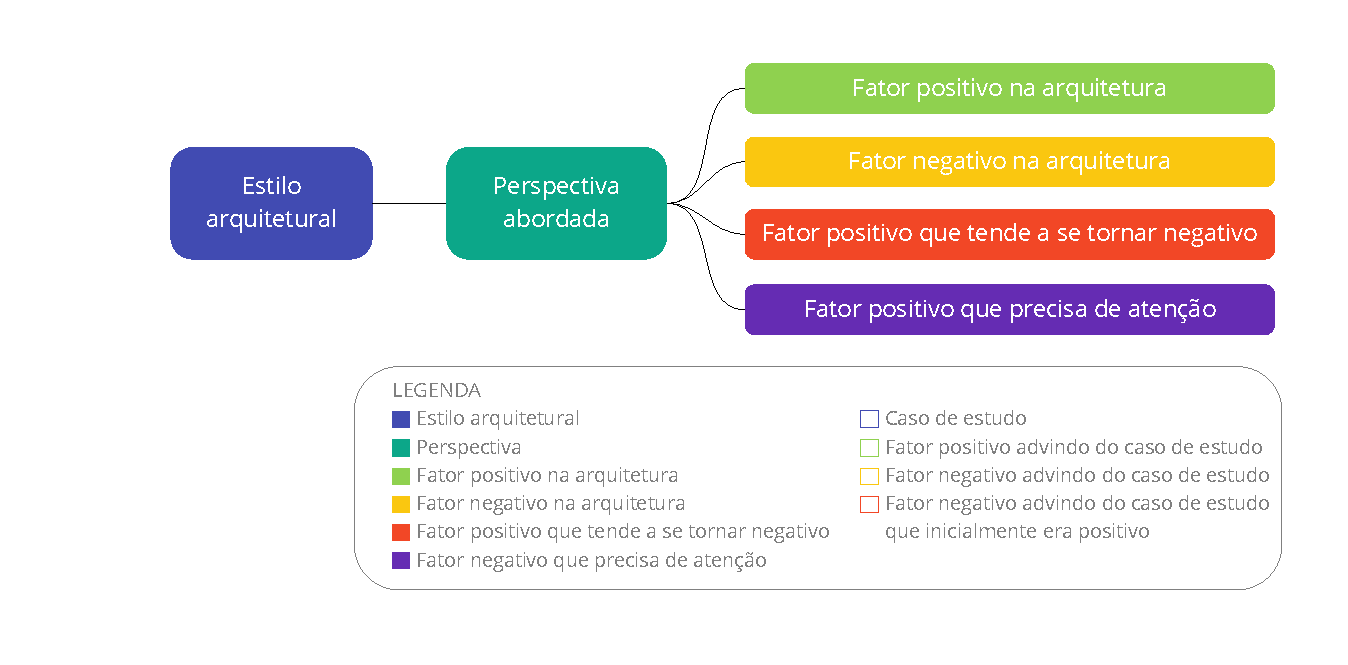
\includegraphics[keepaspectratio=true,scale=0.6]{figuras/modelo-mapa-mental.eps}
  \caption{Modelo de mapa mental utilizado para ilustrar o resultado das sínteses\label{fig:ModeloMapaMental}}
\end{figure}

\begin{description}
    \item[Fatores positivos:] fatores que beneficiam o sistema diante um dado contexto;
    \item[Fatores negativos:] fatores que o modelo arquitetural não provê ou possui alguma limitação;
    \item[Fatores positivos que precisam de atenção:] fatores que são positivos no modelo
        arquitetural mas que precisam de cuidados adicionais para não se tornarem um problema
    \item[Fatores positivos que tendem a se tornar negativos:] fatores que são positivos no modelo
        arquitetural mas que tendem a se tornar um problema a medida que a base de código cresce.
\end{description}

\subsection{Etapa 4 - Estudos de caso}

Com o propósito de enriquecer o presente trabalho e avaliar os aspectos levantados nas etapas
anteriores sob uma concepção prática, nesta etapa visou-se analisar casos reais de empresas que
passaram pelo conflito de escolha arquitetural entre microsserviços e monolíticos. Foram analisados
quatro casos:

\begin{description}
    \item[KN Login:] um sistema monolítico inflado de funcionalidades, no qual a equipe se encontra
        impossibilitada de migrar para uma arquitetura de microsserviços mediante a complexidade
        para fazê-lo;
    \item[Otto:] um sistema monolítico legado que passa pela migração para a arquitetura de
        microsserviços;
    \item[Segment:] um sistema monolítico relativamente novo, que passa pela migração para a
        arquitetura de microsserviços e depois passa por uma nova migração para a arquitetura
        monolítica novamente.
    \item[RuaDois:] uma \textit{startup} que começou a sua arquitetura em microsserviços e depois
        optou por mudar para uma arquitetura monolítica.
\end{description}

Para cada caso foi apresentado o contexto no qual o sistema abordado está inserido, seguido dos
seguintes tópicos:

\begin{enumerate}
    \item \textbf{Problemática da aplicação:} compreensão dos problemas e dificuldades enfrentados
        pela empresa na arquitetura inicialmente escolhida;
    \item \textbf{Solução adotada:} compreensão sobre as decisões tomadas pela empresa mediante os
        problemas enfrentados;
    \item \textbf{Panorama pós-adoção da solução:} compreensão sobre como a solução escolhida
        impactou o desenvolvimento de software dentro da empresa;
    \item \textbf{Análise sobre o caso de estudo:} análise sobre o caso estudado mediante as
        perspectivas e aspectos levantados nas etapas anteriores.
\end{enumerate}

\subsection{Etapa 5 - Análise comparativa final}

Por fim, mediante a base de informações reunidas sobre ambos os estilos arquiteturais nas etapas
anteriores, fez-se uma análise final comparando as duas arquiteturas, passando por suas
características mais básicas até a sua evolução no dia a dia dos engenheiros de software.
